\documentclass[runningheads]{llncs}

\usepackage[T1]{fontenc}
\usepackage[utf8]{inputenc}
\usepackage[spanish,es-nodecimaldot]{babel}
\usepackage{graphicx}
\usepackage{booktabs}
\usepackage{array}
\usepackage{xurl}
\usepackage{listings}

\addto\captionsspanish{%
  \renewcommand{\tablename}{Tabla}%
  \renewcommand{\lstlistingname}{Listado}%
}

\lstdefinelanguage{TurnoLang}{
  morekeywords={AGENDA,RESERVAR,DESDE,HASTA,CANCELAR,LIBRE,LISTAR},
  sensitive=true,
  morestring=[b]"
}
\lstset{basicstyle=\ttfamily\small,keywordstyle=\bfseries,
  columns=fullflexible,keepspaces=true,showstringspaces=false,
  breaklines=true,frame=single,aboveskip=6pt,belowskip=6pt}

\begin{document}

\title{TurnoLang: Diseño e Implementación de un Lenguaje Específico de Dominio para la Gestión de Turnos}
\titlerunning{TurnoLang: un DSL para la gestión de turnos}
\author{[NOMBRES DE AUTORES POR CONFIRMAR]}
\authorrunning{Autores por confirmar}
\institute{[INSTITUCIÓN POR CONFIRMAR]\\
\texttt{[CORREOS Y ORCID POR CONFIRMAR]}}
\maketitle

\begin{abstract}
TurnoLang es un lenguaje específico de dominio educativo para describir y
ejecutar reservas sobre una única agenda, un único recurso y un único día. El
proyecto implementa una cadena completa de procesamiento: análisis léxico con
Flex, análisis sintáctico con Bison, construcción de un árbol de sintaxis
abstracta mínimo, validación semántica con estado e interpretación. El diseño
separa los diagnósticos de las salidas funcionales y comparte un único
recorrido de backend para validar, aplicar cambios y observar resultados. La
evaluación automatizada comprende 68 comprobaciones: 5 de proceso y humo, 23
del frontend, 21 semánticas, 15 del intérprete y 4 de calidad y
reproducibilidad. En el entorno verificado, todas aprobaron. El resultado es un
intérprete pequeño y reproducible que permite estudiar de forma trazable las
fases clásicas de un compilador, con limitaciones explícitas de alcance y de
verificación dinámica de memoria.

\keywords{Lenguaje específico de dominio \and Compiladores \and Flex \and
Bison \and Análisis semántico \and Intérprete}
\end{abstract}

\section{Introducción}

Los lenguajes específicos de dominio (DSL) restringen su vocabulario y sus
operaciones a un problema delimitado. Esa especialización puede mejorar la
expresividad dentro del dominio, aunque exige justificar el costo de diseñar,
implementar y mantener una nueva notación \cite{mernik2005dsl}. TurnoLang fue
concebido como un caso académico acotado: reemplazar instrucciones manuales
ambiguas por órdenes que puedan validarse antes de alterar una agenda, sin
incorporar persistencia, fechas, múltiples recursos ni interfaz gráfica.

El objetivo principal no es reemplazar un sistema de turnos real, sino hacer
observable el recorrido completo que transforma texto fuente en efectos
controlados. El proyecto materializa las fases habituales de un procesador de
lenguajes: reconocimiento de tokens, análisis gramatical, representación
intermedia, comprobaciones contextuales y ejecución \cite{aho2012compilers}.
Además, incorpora una batería reproducible que verifica códigos de salida,
salida estándar y diagnósticos completos.

Las contribuciones del trabajo son: (1) una sintaxis pequeña y coherente para
reservar, cancelar, consultar disponibilidad y listar; (2) un AST que conserva
tipo, datos, línea y orden; (3) un motor semántico con estado y un único
recorrido de backend; y (4) evidencia automatizada de 68 comprobaciones. El
resto del artículo presenta los fundamentos, el diseño, la arquitectura, la
implementación, la evaluación y las limitaciones.

\section{Fundamentos y Decisiones de Diseño}

La separación entre análisis léxico, sintáctico y semántico sigue la
organización clásica de un frontend de compilador \cite{aho2012compilers}. En
TurnoLang, Flex genera el scanner a partir de expresiones regulares; su manual
define este modelo de reglas compuestas por patrones y acciones
\cite{flex2016}. Bison genera el parser LR y permite asociar acciones a las
producciones, además de destructores para liberar valores descartados durante
el análisis \cite{bison2021}.

Se adoptó una sintaxis textual imperativa porque permite mostrar con claridad
la diferencia entre forma y significado. Por ejemplo, \texttt{25:70} respeta
el patrón léxico \texttt{HH:MM} y la gramática de una hora, pero es inválido en
la fase semántica. Esta decisión evita duplicar rangos numéricos en el scanner
y hace visible la responsabilidad de cada etapa.

El dominio se restringe deliberadamente. Un programa declara exactamente una
agenda y luego contiene cero o más instrucciones. El estado existe solo durante
la ejecución. Los intervalos son semiabiertos $[inicio, fin)$: dos reservas
consecutivas, como 09:00--09:30 y 09:30--10:00, no se superponen. Una
cancelación desactiva la reserva, libera su intervalo y permite reutilizar el
identificador.

Los programas usan la extensión \texttt{.tl}. Una cadena de agenda se escribe
entre comillas dobles y no cruza líneas; los identificadores comienzan con letra
o guion bajo y continúan con letras, dígitos o guiones bajos; y un horario tiene
exactamente dos dígitos, dos puntos y dos dígitos. El rango numérico del horario
se comprueba después, durante el análisis semántico.

\section{Lenguaje y Gramática}

La Tabla~\ref{tab:instrucciones} resume las construcciones del lenguaje. Todas
las palabras reservadas distinguen mayúsculas y minúsculas, y cada sentencia
termina con punto y coma.

\begin{table}
\caption{Instrucciones y efectos de TurnoLang.}
\label{tab:instrucciones}
\centering
\small
\begin{tabular}{p{0.27\textwidth}p{0.64\textwidth}}
\toprule
\textbf{Construcción} & \textbf{Semántica} \\
\midrule
\texttt{AGENDA "nombre";} & Declara el nombre no vacío de la agenda. \\
\texttt{RESERVAR id DESDE h1 HASTA h2;} & Crea una reserva válida, activa y no superpuesta. \\
\texttt{CANCELAR id;} & Desactiva una reserva activa existente. \\
\texttt{LIBRE DESDE h1 HASTA h2;} & Informa disponibilidad sin modificar el estado. \\
\texttt{LISTAR;} & Muestra las reservas activas ordenadas por inicio. \\
\bottomrule
\end{tabular}
\end{table}

La gramática implementada se presenta en el Listado~\ref{lst:gramatica}. El
scanner reconoce por separado cadenas, identificadores y horarios. Los valores
asociados a esos tokens se transfieren al parser para construir el AST.

\begin{lstlisting}[caption={Gramática abstracta de TurnoLang.},label={lst:gramatica}]
programa       ::= cabecera sentencia* EOF
cabecera       ::= AGENDA CADENA ";"
sentencia      ::= reserva | cancelacion | disponibilidad | listado
reserva        ::= RESERVAR IDENT DESDE HORA HASTA HORA ";"
cancelacion    ::= CANCELAR IDENT ";"
disponibilidad ::= LIBRE DESDE HORA HASTA HORA ";"
listado        ::= LISTAR ";"
\end{lstlisting}

El Listado~\ref{lst:programa} ilustra un programa que reserva, consulta,
cancela, vuelve a consultar y finalmente lista. La salida funcional se produce
solo para \texttt{LIBRE} y \texttt{LISTAR}; reservar y cancelar no imprimen
confirmaciones.

\begin{lstlisting}[language=TurnoLang,caption={Programa válido usado en la demostración.},label={lst:programa}]
AGENDA "Consultorio Integral";
RESERVAR turno1 DESDE 09:00 HASTA 09:30;
LIBRE DESDE 09:15 HASTA 09:45;
CANCELAR turno1;
LIBRE DESDE 09:00 HASTA 09:30;
RESERVAR turno2 DESDE 10:00 HASTA 10:30;
RESERVAR turno3 DESDE 08:00 HASTA 08:30;
LISTAR;
\end{lstlisting}

\section{Arquitectura}

La Figura~\ref{fig:arquitectura} muestra el flujo principal, desde el archivo
fuente hasta la salida. El diagrama es lineal para enfatizar que el backend no
reanaliza el texto: consume la representación producida por el frontend. Cada
caja identifica una responsabilidad y las flechas representan la transferencia
de tokens, nodos o efectos.

\begin{figure}
\centering
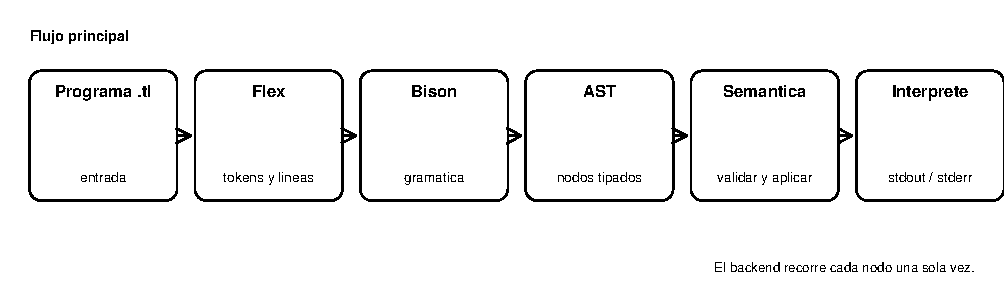
\includegraphics[width=\textwidth]{figuras/arquitectura.pdf}
\caption{Arquitectura de procesamiento de TurnoLang.}
\label{fig:arquitectura}
\end{figure}

El parser no ejecuta instrucciones. Construye una lista enlazada tipada que
conserva el orden del programa. Como se anticipa en la
Figura~\ref{fig:ast}, la raíz almacena el nombre de agenda y los extremos de la
lista. Cada nodo contiene el tipo, la línea de origen, una unión con los datos
de su variante y un enlace al siguiente nodo.

\begin{figure}
\centering
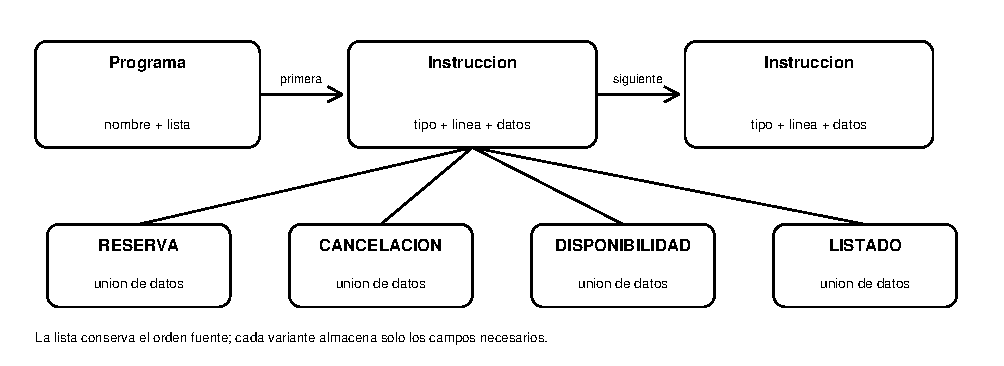
\includegraphics[width=\textwidth]{figuras/ast_minimo.pdf}
\caption{Estructura mínima del AST y variantes de instrucción.}
\label{fig:ast}
\end{figure}

La agenda se encapsula detrás de una interfaz. Su lista enlazada guarda copias
de los identificadores y el intervalo convertido a minutos. Para listar, el
módulo expone un arreglo temporal de vistas de las reservas activas, ordenado
por inicio y, como desempate defensivo, por identificador. Así, el intérprete no
depende de la estructura privada de los nodos.

\section{Implementación}

\subsection{Frontend con Flex y Bison}

El archivo \texttt{lexer.l} prioriza palabras reservadas antes que
identificadores y clasifica errores específicos: cadenas sin cierre, horarios
mal formados, lexemas numéricos no admitidos y caracteres desconocidos. Los
mensajes incluyen la línea y el lexema. Un indicador evita que un error léxico
genere además un diagnóstico sintáctico secundario.

El archivo \texttt{parser.y} especifica la gramática, construye nodos mediante
funciones del módulo AST y transfiere la raíz aceptada al programa principal.
Los destructores de Bison liberan textos y subárboles abandonados. Esta política
es coherente con las facilidades documentadas para símbolos semánticos
\cite{bison2021} y permite que cada bloque tenga un propietario identificable.

El Listado~\ref{lst:frontend} reproduce la regla Flex para la palabra reservada
\texttt{RESERVAR} y la producción Bison que toma los valores del identificador
y de ambas horas. La acción crea directamente el nodo mínimo y conserva la
línea del primer símbolo.

\begin{lstlisting}[caption={Regla Flex y producción Bison reales para una reserva.},label={lst:frontend}]
"RESERVAR" { DEVOLVER_TOKEN(TOK_RESERVAR); }

reserva:
  TOK_RESERVAR TOK_IDENT TOK_DESDE TOK_HORA
  TOK_HASTA TOK_HORA TOK_PUNTO_Y_COMA
  {
    $$ = ast_reserva_crear($2, $4, $6, @1.first_line);
  }
;
\end{lstlisting}

\subsection{AST, Semántica e Intérprete}

El AST es intencionalmente pequeño: no conserva tokens de puntuación ni
palabras reservadas, solo información necesaria para las etapas siguientes. La
línea de cada instrucción se copia al nodo para producir diagnósticos sin volver
al texto fuente.

Antes de recorrer el programa, cada horario válido se transforma a minutos
mediante $60 \times hora + minuto$. La superposición se decide con la condición
real del Listado~\ref{lst:superposicion}. \texttt{inicio\_a} y
\texttt{fin\_a} describen el intervalo nuevo; \texttt{inicio\_b} y
\texttt{fin\_b}, una reserva activa existente. Las desigualdades estrictas
implementan intervalos semiabiertos y permiten extremos consecutivos.

\begin{lstlisting}[language=C,caption={Condición implementada para detectar superposición.},label={lst:superposicion}]
return inicio_a < fin_b && fin_a > inicio_b;
\end{lstlisting}

El motor \texttt{semantica\_procesar\_programa} recorre la lista una sola vez.
Para cada nodo aplica la secuencia \emph{validar, aplicar y observar}. La
validación comprueba horarios entre 00:00 y 23:59, intervalos no vacíos y
crecientes, identificadores activos únicos, ausencia de superposición y
existencia de reservas al cancelar. Solo después del éxito se modifica la
agenda. Un observador opcional recibe la instrucción ya aplicada: el modo de
solo semántica usa el motor sin observador, mientras que la interpretación
instala uno para \texttt{LIBRE} y \texttt{LISTAR}.

Esta organización evita dos agendas y dos recorridos independientes. Ante el
primer error semántico, la instrucción rechazada y las posteriores no se
ejecutan. En cambio, las salidas funcionales generadas por instrucciones
anteriores permanecen en \texttt{stdout}. Si el frontend falla, el backend no
comienza, aunque el error aparezca tarde en el archivo.

\subsection{Construcción Reproducible}

El \texttt{Makefile} declara las dependencias entre el archivo de Bison, su
encabezado, el scanner generado, los objetos y el ejecutable. GNU Make determina
qué objetivos requieren actualización según sus dependencias y marcas de
tiempo \cite{make2023}. El proyecto admite \texttt{make}, \texttt{make -j2},
\texttt{make test} y \texttt{make clean}; este último elimina solo artefactos
generados. La compilación verificada utiliza opciones C11 y advertencias
\texttt{-Wall -Wextra -Wpedantic}.

La propiedad de memoria se distribuye de forma explícita: Flex reserva los
textos; los constructores del AST toman su propiedad; la agenda copia los
identificadores; el arreglo temporal de listado contiene vistas; y el programa
principal libera AST, scanner y archivo. Las rutas de error liberan el estado
construido hasta ese punto.

\section{Evaluación}

La evaluación se ejecutó el 2 de noviembre de 2026 en Windows 11 con Git Bash,
Flex 2.6.4 (\texttt{winflexbison} 2.5.25), Bison 3.8.2, GCC 15.2.0, GNU Make
4.4.1 y Bash 5.3.15. La Tabla~\ref{tab:resultados} presenta el resultado real de
\texttt{make test} después de una construcción limpia.

\begin{table}
\caption{Resultado de la batería integral.}
\label{tab:resultados}
\centering
\small
\begin{tabular}{l@{\hspace{1.2em}}r@{\hspace{1.2em}}r@{\hspace{1.2em}}r}
\toprule
\textbf{Suite} & \textbf{Pruebas} & \textbf{Aprobadas} & \textbf{Fallidas} \\
\midrule
Proceso y humo & 5 & 5 & 0 \\
Frontend & 23 & 23 & 0 \\
Semántica & 21 & 21 & 0 \\
Intérprete & 15 & 15 & 0 \\
Calidad y reproducibilidad & 4 & 4 & 0 \\
\midrule
\textbf{Total} & \textbf{68} & \textbf{68} & \textbf{0} \\
\bottomrule
\end{tabular}
\end{table}

Las pruebas del frontend distinguen aceptación sintáctica y rechazo léxico o
gramatical. Las semánticas cubren rangos, orden de intervalos, duplicados,
superposiciones parciales y contenidas, cancelaciones, reutilización y límites
horarios. Las funcionales comparan código de salida, \texttt{stdout} y
\texttt{stderr} completos contra oráculos versionados, e incluyen orden,
agenda vacía, continuidad tras consultas y bloqueo del backend ante fallos del
frontend.

Las cuatro comprobaciones de calidad agregan archivo vacío, archivo válido sin
salto final, ruta con espacios y una falla inducida del comparador. Esta última
confirma que el runner detecta un oráculo alterado en vez de limitarse a mostrar
un resumen exitoso. La normalización se restringe a terminadores CRLF/LF para
comparar la salida del ejecutable nativo de Windows con los oráculos del
repositorio.

La ejecución completa del Listado~\ref{lst:programa} produjo dos consultas de
disponibilidad y un listado ordenado con \texttt{turno3} antes de
\texttt{turno2}. El resultado coincide exactamente con el oráculo versionado.
Asimismo, los casos de horario \texttt{9:30}, sentencia sin punto y coma y
superposición generan, respectivamente, errores léxico, sintáctico y
semántico con código de salida 1.

\section{Limitaciones y Amenazas a la Validez}

El alcance funcional es deliberadamente reducido: una agenda, un recurso, un
día y estado volátil. No se implementaron fechas, persistencia, concurrencia,
zonas horarias, autenticación, interfaz gráfica ni recuperación para continuar
después de un error. Por ello, el resultado no debe interpretarse como un
sistema de reservas listo para producción.

La evidencia de ejecución corresponde al entorno Windows descrito. No se
declara compatibilidad verificada con otros sistemas. Valgrind no estaba
disponible; el GCC MinGW instalado carecía de \texttt{libasan} y
\texttt{libubsan}; WSL Ubuntu no estaba instalado; y el motor Docker no estaba
activo. Se ejecutó \texttt{GCC -fanalyzer}: los módulos propios no produjeron
advertencias, mientras que el código generado requirió distinguir rutas de las
herramientas. La ausencia de una ejecución dinámica de memoria en Linux sigue
siendo una limitación y no se sustituye por la revisión estática.

Las 68 comprobaciones son deterministas y cubren las reglas documentadas, pero
no constituyen una demostración formal ni una medición exhaustiva de todas las
entradas posibles. Además, la defensa oral todavía requiere un ensayo humano
cronometrado y los metadatos de autoría deben completarse antes de considerar
este manuscrito definitivo.

\section{Conclusiones}

TurnoLang demuestra una cadena completa y trazable desde texto fuente hasta
ejecución. La separación de responsabilidades permite observar dónde se decide
la validez léxica, sintáctica y semántica, mientras que el AST desacopla el
frontend del backend. El recorrido compartido \emph{validar, aplicar y
observar} evita duplicación entre el modo semántico y el intérprete.

La construcción limpia y las 68 comprobaciones aprobadas aportan evidencia
reproducible del comportamiento implementado. El principal trabajo pendiente
antes de la entrega definitiva es administrativo y de validación final:
completar autores, afiliación, correos y, si corresponde, ORCID; realizar el
ensayo humano dentro de los 15 minutos; y, cuando exista un entorno Linux
adecuado, complementar la revisión de memoria con Valgrind o sanitizers.

El documento utiliza la clase y el estilo bibliográfico oficiales de LNCS. La
preparación siguió las instrucciones de Springer para autores, en particular la
referencia cruzada de figuras y tablas, el uso de gráficos vectoriales y la
correspondencia entre citas y bibliografía \cite{springer2026lncs}.

\bibliographystyle{splncs04}
\bibliography{referencias}

\end{document}
